\chapter{The \cls{MRTbeam} class}
The \cls{MRTbeam} class is a class build upon \cls{beamer}. It should mimic the
style of the MS Powerpoint template of the MRT which was in use when I held my
Bachelor's presentation. I heard the requirements to match a specific
template are less strict today, but at least I'll still use this template.

Many of the features described here are also available if one uses
\cs{usetheme{MRTbeam}} within a document using the \cls{beamer} class. There
however is no dedicated documentation for that possibility provided. You're
encouraged to also use the corresponding \cls{MRTbeam} class if your using the
eponymous theme.

If there is a new institution template which should be matched that doesn't
match this \cls{beamer} template please contact me as described in
\autoref{sec:bugs}.

\section{Random chatter}
The creation of a presentation using \cls{beamer} is not everyone's cup of tea.
Refer to the \cls{beamer} manual to get a basic idea of how to use it, as
\cls{MRTbeam} only adds some stuff that is not basic \cls{beamer} stuff. The
main idea of creating a presentation remains that of \cls{beamer}.

\cls{MRTbeam} doesn't follow the way \cls{beamer} does things everywhere. As a
result some stuff may not work out as you expect if you're used to \cls{beamer}.
Especially the customization might require you to actually read the sources of
\cls{MRTbeam} and its beamer themes. Also \cls{MRTbeam} is only for presentation
mode as of now.

Special thanks are due to the TeX.SX user samcarter, who helped me ram my head
through \cls{beamer}'s walls in order to get my will.

\section{Frame contents}
The class builds up frames as shown in \autoref{fig:beam:frame} (not true to
scale).
\begin{figure}[!bp]
  \centering
  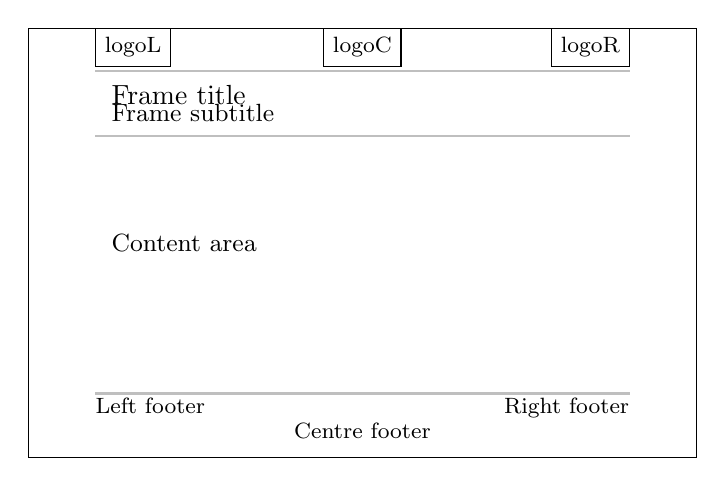
\begin{tikzpicture}[x=.7\textwidth,y=.45\textwidth]
    \draw (0,0) rectangle (1,1);
    \node[anchor=south west,draw] at (.1,.91) {\footnotesize logoL};
    \node[anchor=south,draw] at (.5,.91) {\footnotesize logoC};
    \node[anchor=south east,draw] at (.9,.91) {\footnotesize logoR};
    \draw[color=white!75!black,thick] (.1,.9) -- (.9,.9);
    \node[anchor=north west] at (.11,.89) {Frame title};
    \node[anchor=south west] at (.11,.76) {\small Frame subtitle};
    \draw[color=white!75!black,thick] (.1,.75) -- (.9,.75);
    \node[anchor=west] at (.11,.5) {\small Content area};
    \draw[color=white!75!black,thick] (.1,.15) -- (.9,.15);
    \footnotesize
    \node[anchor=north west,inner sep=0] at (.1,.14) {Left footer};
    \node[anchor=north] at (.5,.1) {Centre footer};
    \node[anchor=north east,inner sep=0] at (.9,.14) {Right footer};
  \end{tikzpicture}
  \caption{The basic layout of a frame in \cls{MRTbeam}}
  \label{fig:beam:frame}
\end{figure}

You can specify the used logos using \cs{uselogo}. The default is the UBT logo
on the left, no logo in the centre, and the MRT logo on the right side.

If you specify no or an empty frame title the current section is used (with its
numbering). The frame's subtitle can be prepended with the current subsection
(with its numbering) followed by a colon. This depends on the current value of
\cs{ifPrependSubsections}.

The left footer contains the \texttt{occasion}, the \texttt{shorttitle}, and the
\texttt{shortauthor}. If no short title or no short author is given, the title
and the author, respectively, are used instead. If you give a \texttt{*} for the
short author or the short title, they are left out (e.g. with using
\verb|\title[*]{foo}|).

The centre footer contains the frame number and if you want a progress bar. The
progress bar is shown if \cs{ifProgressBar} is true.

In the right footer the following is displayed atop of each other: Persistent
MRT footnotes, volatile MRT footnotes, citation MRT footnotes, normal footnotes.
The right footer has enough space for three entries. If you need more they are
scaled to the available vertical space. MRT footnotes might be displayed in a
tabular manner with the labels in the left and the actual notes in the right
column. This depends on the value of \cs{ifTabularNotes}.

Neither of the footers is restricted in horizontal size. As a result they might
overlap if you specify really long contents.

\section{Options}
The class passes all options given to it on to \cls{beamer}. There are still
some class specific options which you can set with some macros. The macros in
this section are only provided to set specific options, other macros are
described in \autoref{sec:beam:macros}.

\begin{describemacro}{advisor}[\meta{*}\oarg{title}\marg{name}]
  Sets \meta{name} as the current advisor. It also redefines itself, any
  consecutive call will not take any arguments but return the \meta{name}. The
  \meta{title} shall be the title used on the title frame defaulting to
  \enquote{Betreuerin} if the starred version is used, else it defaults to
  \enquote{Betreuer}.
\end{describemacro}

\begin{describemacro}{occasion}[\marg{occasion}]
  Defines the occasion of the presentation. If used the occasion will be
  displayed in the left footer.
\end{describemacro}

\begin{describemacro}{uselogo}[\marg{pos}\oarg{options}\marg{file}]
  Specifies the logo used at the position \meta{pos}. There are \texttt{l},
  \texttt{c}, and \texttt{r} available. The \meta{file} is included using
  \cs{includegraphics} with the specified \meta{options} (defaulting to
  \texttt{height=0.056\cs{paperwidth}}). If \meta{file} is an empty argument
  there is no logo used at the specified position. By default
  \file{MRTbeam_logo_UBT2.pdf} is used for the left logo and
  \file{MRTbeam_logo_MRT2.pdf} for the right one. The centre logo is initially
  empty.
\end{describemacro}

\begin{describemacro}{ShowGrid}[\oarg{options}]
  Globally activates a \TikZ\ grid displayed in the background of the frames.
  You can specify the \TikZ-style used for the grid with \meta{options}. The
  default is: \verb|xstep=.05\paperwidth, ystep=.1\paperheight, help lines|.
\end{describemacro}

\begin{describemacro}{HideGrid}[\meta{*}]
  Globally deactivates the background grid and restores the package's default
  options for that grid. If the starred version is used, the options are not
  reset.
\end{describemacro}

\begin{describemacro}
  {ifPrependSubsections,PrependSubsectionstrue,PrependSubsectionsfalse}
  If set true each \env{frame}'s subtitle is prepended by the current
  subsection.
\end{describemacro}

\begin{describemacro}{ifOnlyOneTopRule,OnlyOneTopRuletrue,OnlyOneTopRulefalse}
  If set true in each \env{frame} the title and subtitle will not be displayed
  and the lower top rule will be omitted, significantly enlarging the content
  area. If you use \cs{OnlyOneTopRuletrue} or \cs{OnlyOneTopRulefalse}
  \cs{contentheight} will be adjusted.
\end{describemacro}

\begin{describemacro}{ifProgressBar,ProgressBartrue,ProgressBarfalse}
  If set true a progress bar will be shown in the middle of the slides foot at
  the frame number. You can customize the progress bar shown using
  \cs{SetProgressBar} or \cs{ProgressBarStyle}.
\end{describemacro}

\begin{describemacro}{SetProgressBar}%
  [\meta{*}\marg{align}\marg{length}\marg{height}\marg{voffset}]
  This changes the default values of \cs{ProgressBar}. If the starred version is
  used the changes are made locally, else they are applied globally. Take a look
  at the description of \cs{ProgressBar} for an explanation what each of the
  parameters mean. If you use a \texttt{*} as one of the arguments the
  corresponding default value will remain unchanged.
\end{describemacro}

\begin{describemacro}{ProgressBarStyle}[\meta{*}\marg{style}]
  This sets the progress bar options to a predefined \meta{style} using the
  unstarred version of \cs{SetProgressBar}. If the starred version of
  \cs{ProgressBarStyle} is used \cs{ProgressBartrue} is issued.\par
  \bigskip
  \noindent
  \small
  \MRTtabDeclareHeadMacros
  \setstretch{1.408}%
  \begin{tabularx}{\textwidth}{l*4c>{\setstretch{1}}X}
    \headS
    style & align & length & height & voffset & description\\
    \headE
    default & c & 30pt            & font size & -1.65ex
      & a thick and relatively short bar around the frame number\\
    Spratte & c & \cs{paperwidth} & 2pt       & 3pt
      & A thin line spanning the whole page width at the bottom of the frame\\
    \hline
  \end{tabularx}
\end{describemacro}

\subsection{Footnote related}
\begin{describemacro}{ifTabularNotes,TabularNotestrue,TabularNotesfalse}
  If set true the MRT footnotes will be displayed in a tabular manner with two
  columns. MRT footnotes are those footnotes set with the footnote related
  macros in \autoref{sec:beam:macros:foot}.
\end{describemacro}

\begin{describemacro}{ColumnsTabularNotes}[\marg{specification}]
  With this macro you can specify the column specifications used by MRT
  footnotes. Your definition should contain two columns.
\end{describemacro}

\subsection{Bibliography related}
\begin{describemacro}
  {ifExplicitCiteOnce,ExplicitCiteOncetrue,ExplicitCiteOncefalse}%
  If set to true for every used key the citation is in an explicit manner only
  once. For each following citation of the same key only the number is used.
\end{describemacro}

\begin{describemacro}{ifNoExplicitCite,NoExplicitCitetrue,NoExplicitCitefalse}
  If set to true there will never be an explicit citation at the frame, only the
  citation number will be used.
\end{describemacro}

\section{Macros}\label{sec:beam:macros}
\begin{describemacro}{PlaceAt}%
  [\meta{*}\barg{pos}\oarg{node options}\marg{content}]
  The starred version differs fundamentally from the unstarred one. The
  unstarred one places \meta{content} at the specified position \meta{pos} in
  the background inside a \TikZ\ node with the optionally specified \meta{node
  options}. The coordinates default to multiples of \cs{pagewidth} and
  \cs{pageheight} for \texttt{x} and \texttt{y}, respectively. You can use
  anything \TikZ\ understands as coordinates for \meta{pos}.\\[\parskip]
  The starred version places the \env{tikzpicture} where you currently are. It
  uses \texttt{remember picture} and \texttt{overlay} as options. The \meta{pos}
  must match the pattern \carg{x}{y}. \meta{x} is in multiples of \cs{pagewidth}
  and \meta{y} in multiples of \cs{pageheight} and you can't change that. The
  node still gets \meta{node options}.\\[\parskip]
  In both cases \texttt{(0,0)} is the bottom left corner of the slide.
\end{describemacro}

\begin{describemacro}{AddToPlaced}[\marg{tikz code}]
  Adds the specified \meta{tikz code} to the background of the current slide.
  \texttt{(0,0)} is the bottom left corner of the slide. Coordinates are by
  default in multiples of \cs{pagewidth} and \cs{pageheight}. It uses the same
  \env{tikzpicture} as \cs{PlaceAt} and is stored in the same macro.
\end{describemacro}

\begin{describemacro}{ProgressBar}%
  [\oarg{align}\sarg{length}\oarg{height}\oarg{voffset}]
  Prints a progress bar. \meta{align} is the horizontal alignment as you would
  pass it to a \cs{makebox}, the initial default is \texttt{c}. \meta{length} is
  the overall length the progress bar should have (defaulting to \texttt{30pt}),
  \meta{height} its height, defaulting to the current font size. \meta{voffset}
  allows you to offset the progress bar vertically. With positive values the
  shift is downwards, the default is \texttt{-1.65ex}. The progress bar uses the
  \pkg{xcolor} colours \texttt{progressed} and \texttt{noprogress}. All
  arguments are optional.
\end{describemacro}

\begin{describemacro}{StartOfProgress,EndOfProgress}
  Denotes the start and end of the progress bars gauge. The \env{frame} after
  the call of \cs{StartOfProgress} is the first \env{frame} filling the gauge,
  the \env{frame} prior to \cs{EndOfProgress} is the first \env{frame} in which
  the gauge is fully filled. The macros should be used outside of the
  \env{frame} environment. If \cs{StartOfProgress} is not used the first
  \env{frame} starts filling the gauge, if \cs{EndOfProgress} is not used the
  last \env{frame} is the only one with a completely filled gauge.
\end{describemacro}

\begin{describemacro}{contentwidth,contentheight}
  These are lengths which are set to match the height and width of the content
  block of a \env{frame} (the space between the bottom rule and the lower top
  rule). \cs{textwidth} should match \cs{contentwidth} if you're outside of a
  \env{minipage} or similar, but \cs{textheight} will most likely not match the
  actual height of the content area.
\end{describemacro}

\begin{describemacro}{UseAndIfEmptyTF}%
  [\oarg{pre}\marg{arg}\marg{true}\marg{false}]
  The \meta{arg} is expanded inside a box. If that box has a width not equal 0pt
  \meta{pre} is used followed by the contents of the box. Then the \meta{false}
  branch is executed. If the box's width equals 0pt the \meta{true} branch is
  used instead and neither \meta{pre} is used nor the box containing \meta{arg}
  placed.
\end{describemacro}

\begin{describemacro}{cursec}[\meta{*}]
  If the current section is starred or you used the optional \texttt{*} for
  \cs{cursec}, this macro inserts the current sections name, else the name is
  prepended by the current sections number.
\end{describemacro}

\begin{describemacro}{curssec}[\meta{*}]
  This macro is very similar to \cs{cursec}. If you used the starred version of
  it or the current subsection is starred, this macro inserts the current
  subsections name, else the name is prepended by the current subsections
  number.
\end{describemacro}

\begin{describeenv}{whiteframes}
  In this environment \cs{ifwhiteframes} is set true.
\end{describeenv}

\subsection{Footnote related}\label{sec:beam:macros:foot}
The term footnotes relates to the special MRT footnotes in this section.
\begin{describemacro}{AddToRightFoot}%
  [\meta{*}\meta{+}\sarg{overlay}\oarg{pre}\marg{note}]
  This macro adds stuff to the right footer. If \meta{*} is given, the content
  is added to the persistent footnotes, else if \meta{+} is given added to the
  cite related footnotes, else to the ordinary ones. \meta{overlay} is used for
  any overlay specifications using \cs{uncover}. \meta{pre} is added left to
  \meta{note}. If tabular footnotes are used \meta{pre} is in the left,
  \meta{note} in the right column. If tabular footnotes are not used the
  distance between \meta{pre} and \meta{note} is \texttt{0.5}\cs{tabcolsep}. The
  starred variant should only be used outside of the \env{frame} environment. If
  you get strange errors during compilation a \cs{noexpand} in front of some
  macros (e.g. stuff like \cs{href}) you give as arguments might help.
\end{describemacro}

\begin{describemacro}{ClearRightFoot}[\meta{*}]
  Clears the footnotes. If the \texttt{*} is given only the volatile footnotes
  are cleared, else all of them.
\end{describemacro}

\subsection{Bibliography related}
\begin{describemacro}{cite}[\sarg{overlay}\oarg{opt1}\oarg{opt2}\marg{key}]
  \meta{overlay} is handled by \cs{uncover}, which affects only the footnote not
  the footnote mark. The usage of the two optional arguments and \meta{key}
  match those known from \pkg{biblatex}'s \cs{cite}. The citation's contents are
  dependent on \cs{ifNoExplicitCite} and \cs{ifExplicitCiteOnce}, an explicit
  citation contains the citation number, authors' names, the journal, and the
  year.
\end{describemacro}

\begin{describemacro}{framecite}%
  [\meta{*}\sarg{overlay}\oarg{pre}\marg{key}\oarg{post}]
  Places a citation in the footnotes, if the starred version is used using the
  persistent footnotes, else the volatile non-cite related footnotes. Use the
  starred version prior to the \env{frame} it should first be shown in.
  \meta{overlay} specifications are interpreted by \cs{uncover}. \meta{pre} is
  put in front of the citation with a distance of \cs{,} (unaffected by tabular
  footnotes options), \meta{post} with a distance of \cs{,} after the citation.
  The citation contains the authors' names, the journal, and the year.
\end{describemacro}

\begin{describemacro}{bibliographyframe}%
  [\meta{*}\oarg{bibfont}\marg{title}\marg{subtitle}]
  Prints the bibliography. The starred variants uses \cs{whiteframestrue}. The
  \meta{bibfont} defaults to \cs{small}, you might give any font related
  commands here. Both \meta{title} and \meta{subtitle} are optional though
  delimited by curly braces. \meta{title} defaults to \enquote{Quellen},
  \meta{subtitle} is initially empty. The \cs{bibliographyframe} is printed
  using \texttt{allowframebreaks}.
\end{describemacro}

\begin{describemacro}{inlinecite}[\oarg{opt1}\oarg{opt2}\marg{key}]
  Gives the citation which would be placed in the in the text by \cs{cite}
  without any \cs{textcolor}. In fact \cs{cite} uses this internally.
\end{describemacro}

\begin{describemacro}{insertcite}[\marg{key}]
  Gives the citation which would be placed in the footnote by \cs{cite}. In fact
  \cs{cite} uses this internally.
\end{describemacro}

\begin{describemacro}{insertframecite}[\marg{key}]
  Gives the citation which would be placed in the footnote by \cs{framecite}. In
  fact \cs{framecite} uses this internally.
\end{describemacro}

\section{Dependencies}
The class uses \cls{beamer} as its basis. Additional the following packages are
loaded:
\vspace*{-\multicolsep}%
\begin{multicols}{3}
  \begin{itemize}
    \item \pkg{helvet}
    \item \pkg{MRTsfacc}
    \item \pkg{xparse}
    \item \TikZ
    \item \pkg{biblatex}
  \end{itemize}
\end{multicols}
\vspace*{-\multicolsep}%
\pkg{biblatex} uses \texttt{biber} as its backend.
